\documentclass[a4paper,12pt]{report}

% import packages
\usepackage{anuthesis}
\usepackage{ucs}
\usepackage[utf8x]{inputenc}
\usepackage{amsmath}
\usepackage{amsfonts}
\usepackage{amssymb}
\usepackage{amsthm}
\usepackage[australian]{babel}
\usepackage{fontenc}
\usepackage{graphicx}

\usepackage{comment}
\usepackage{mathrsfs}
\usepackage{booktabs}
%\usepackage[dvips]{hyperref}
\usepackage{fancyhdr}
\usepackage{fancyvrb}
\usepackage{subfig}
\usepackage{appendix}
\usepackage[bw,numbered]{mcode}
\usepackage[nottoc,numbib]{tocbibind}
\usepackage[round, sort, numbers, authoryear]{natbib} % for author yr referencing


%%%%%%%%%%%%%%%%%%%%%%%%%%%%%%%%%%%%%%
%             Margins
%%%%%%%%%%%%%%%%%%%%%%%%%%%%%%%%%%%%%%
\usepackage[top=30mm, bottom=30mm ,left=30mm, right=30mm]{geometry}

%%%%%%%%%%%%%%%%%%%%%%%%%%%%%%%%%%%%%%
%     Setting page header format
%%%%%%%%%%%%%%%%%%%%%%%%%%%%%%%%%%%%%%
\pagestyle{fancyplain}
\renewcommand{\sectionmark}[1]{\markright{\thesection\ #1}{}}
\renewcommand{\chaptermark}[1]{\markboth{\chaptername\ \thechapter\ #1}{}}
\fancyhf{}
\lhead{\fancyplain{}{\leftmark}}
\rhead{\fancyplain{}{\rightmark}}
\rfoot{\textbf{\thepage}}

\makeatletter
\def\listoffigures{
\@restonecolfalse\if@twocolumn\@restonecoltrue\onecolumn
 \fi\chapter*{List of Figures\@mkboth{List of Figures}{List of Figures}}
 \@starttoc{lof}\if@restonecol\twocolumn\fi
 }
\makeatother

% fix citations to be IEEE style
\def\citepunct{], [}
\def\citedash{]--[}
% Bibliographical style, IEEEtran for IEEE, natbib for Harvard
\bibliographystyle{anuthesis}

%%%%%%%%%%%%%%%%%%%%%%%%%%%%%%%%%%%%%%
%             Authorship
%%%%%%%%%%%%%%%%%%%%%%%%%%%%%%%%%%%%%%
\def\THETITLE{Low cost DDS based Transceiver for Wireless Communication of low VHF}
\title{\THETITLE}
\def\THEAUTHOR{Zhenzhen Liu}
\author{\THEAUTHOR}
\def\studentID{U5625456}
\def\supervisor{Prof. Gerard Gorg}
\date{\today}

\begin{document}
  \setcounter{secnumdepth}{5}
  \setcounter{tocdepth}{7}
  \linespread{1.2}
  \selectfont
  \pagenumbering{roman}  % first use Roman numerals for page numbers
  
  %%%%%%%%%%%%%%%%%%%%%%%%%%%%%%%
  %         Title Page
  %%%%%%%%%%%%%%%%%%%%%%%%%%%%%%%
  \begin{titlepage}
    %\enlargethispage{2cm}
    \vspace*{\fill}
    \begin{center}

      \makeatletter
      \Huge\textbf{\THETITLE} \\[1.5cm]
      \huge\textbf{\THEAUTHOR\ \\ \studentID} \\[1.5cm]
      \Large\textbf{Supervised by \supervisor} \\[1.5cm]
      \thismonth
      \makeatother
      
      \vspace*{\fill}
      
\includegraphics[width=70mm]{images/logo} \\[2cm]
      \vspace*{-1.5cm}
      \Large A thesis submitted in part fulfilment of the degree of \\[0.5cm]
      \LARGE Bachelor of Engineering\\
      The Department of Engineering\\
      Australian National University \\ [0.8cm]      
    \end{center}
    \vspace*{\fill}
  \end{titlepage}

  % include statements effectively insert the contents of the named file.
  % They are not necessary, but are useful for organising your work.
  % They always start a  new page.
  
  %%%%%%%%%%%%%%%%%%%%%%%%%%%%%%%
  %         Plagerism
  %%%%%%%%%%%%%%%%%%%%%%%%%%%%%%%
  \begin{titlepage}
\vspace*{\fill}
\noindent
This thesis contains no material which has been accepted for the award of any other degree or diploma in any university. To the best of the author’s knowledge, it contains no material previously published or written by another person, except where due reference is made in the text.
\\
\\
\\
\\
\hspace*{\fill}\THEAUTHOR \\
\hspace*{\fill}\today
	\vspace*{\fill}
\begin{center}
	\copyright\THEAUTHOR
\end{center}

\end{titlepage}

  %%%%%%%%%%%%%%%%%%%%%%%%%%%%%%%
  %       Acknowledgements
  %%%%%%%%%%%%%%%%%%%%%%%%%%%%%%%
  \chapter*{Acknowledgements}
\addcontentsline{toc}{chapter}{Acknowledgements}

Thanks to my cat, Fluffy and my budgie, Rex.
  % include the contents of the file thanks.tex
  
  %%%%%%%%%%%%%%%%%%%%%%%%%%%%%%%
  %         Abstract
  %%%%%%%%%%%%%%%%%%%%%%%%%%%%%%%
  \chapter*{Abstract}
\addcontentsline{toc}{chapter}{Abstract}

\vspace*{2em}
The abstract should be brief (100-150 words) and directed to readers familiar with the broad area of the thesis subject. ``The abstract is of utmost importance for it is read by 10 to 500 times more people than hear or read the entire article. It should not be a mere recital of the subjects covered, replete with such expressions as ``is discussed'' and ``is described.'' It should be a condensation and concentration of the essential qualities of the paper.''  % include the file abstract.tex

  %%%%%%%%%%%%%%%%%%%%%%%%%%%%%%%
  %      Contents Page
  %%%%%%%%%%%%%%%%%%%%%%%%%%%%%%%
  \selectfont
  \tableofcontents
  %\thispagestyle{empty} % no fancyhdr in the contents page

  %%%%%%%%%%%%%%%%%%%%%%%%%%%%%%%
  %      List of Figures
  %%%%%%%%%%%%%%%%%%%%%%%%%%%%%%%
  \listoffigures % makes a list of figures
  \addcontentsline{toc}{chapter}{List of Figures}

  %%%%%%%%%%%%%%%%%%%%%%%%%%%%%%%
  %      List of Tables
  %%%%%%%%%%%%%%%%%%%%%%%%%%%%%%%
  \listoftables  % uncomment this if you have tables
  \addcontentsline{toc}{chapter}{List of Tables}

  %%%%%%%%%%%%%%%%%%%%%%%%%%%%%%%
  %      Abbreviations
  %%%%%%%%%%%%%%%%%%%%%%%%%%%%%%%
  \selectfont
  \chapter*{Glossary of Terms}
\addcontentsline{toc}{chapter}{List of Abbreviations}

\begin{tabular}{p{0.8cm}p{2.5cm}l}
&DDS		& Direct Digital Synthesiser\\
&VHF		& Very High Frequency \\
&ITU		& Internation Telecommunication Union \\
&RF		& Radio Frequency \\




\end{tabular}


  % Change settings for for Thesis body
  \pagenumbering{arabic} % switch to Arabic numerals for page numbers
  \setcounter{page}{1}  % set page number to 1

  %%%%%%%%%%%%%%%%%%%%%%%%%%%%%%%
  %      Thesis Body
  %%%%%%%%%%%%%%%%%%%%%%%%%%%%%%%
  \chapter{Introduction}
\vspace{-1.4em}

%\begin{figure}[ht]
 %\begin{center}
%trim option's parameter order: left bottom right top, remove square brackets for no trim
 %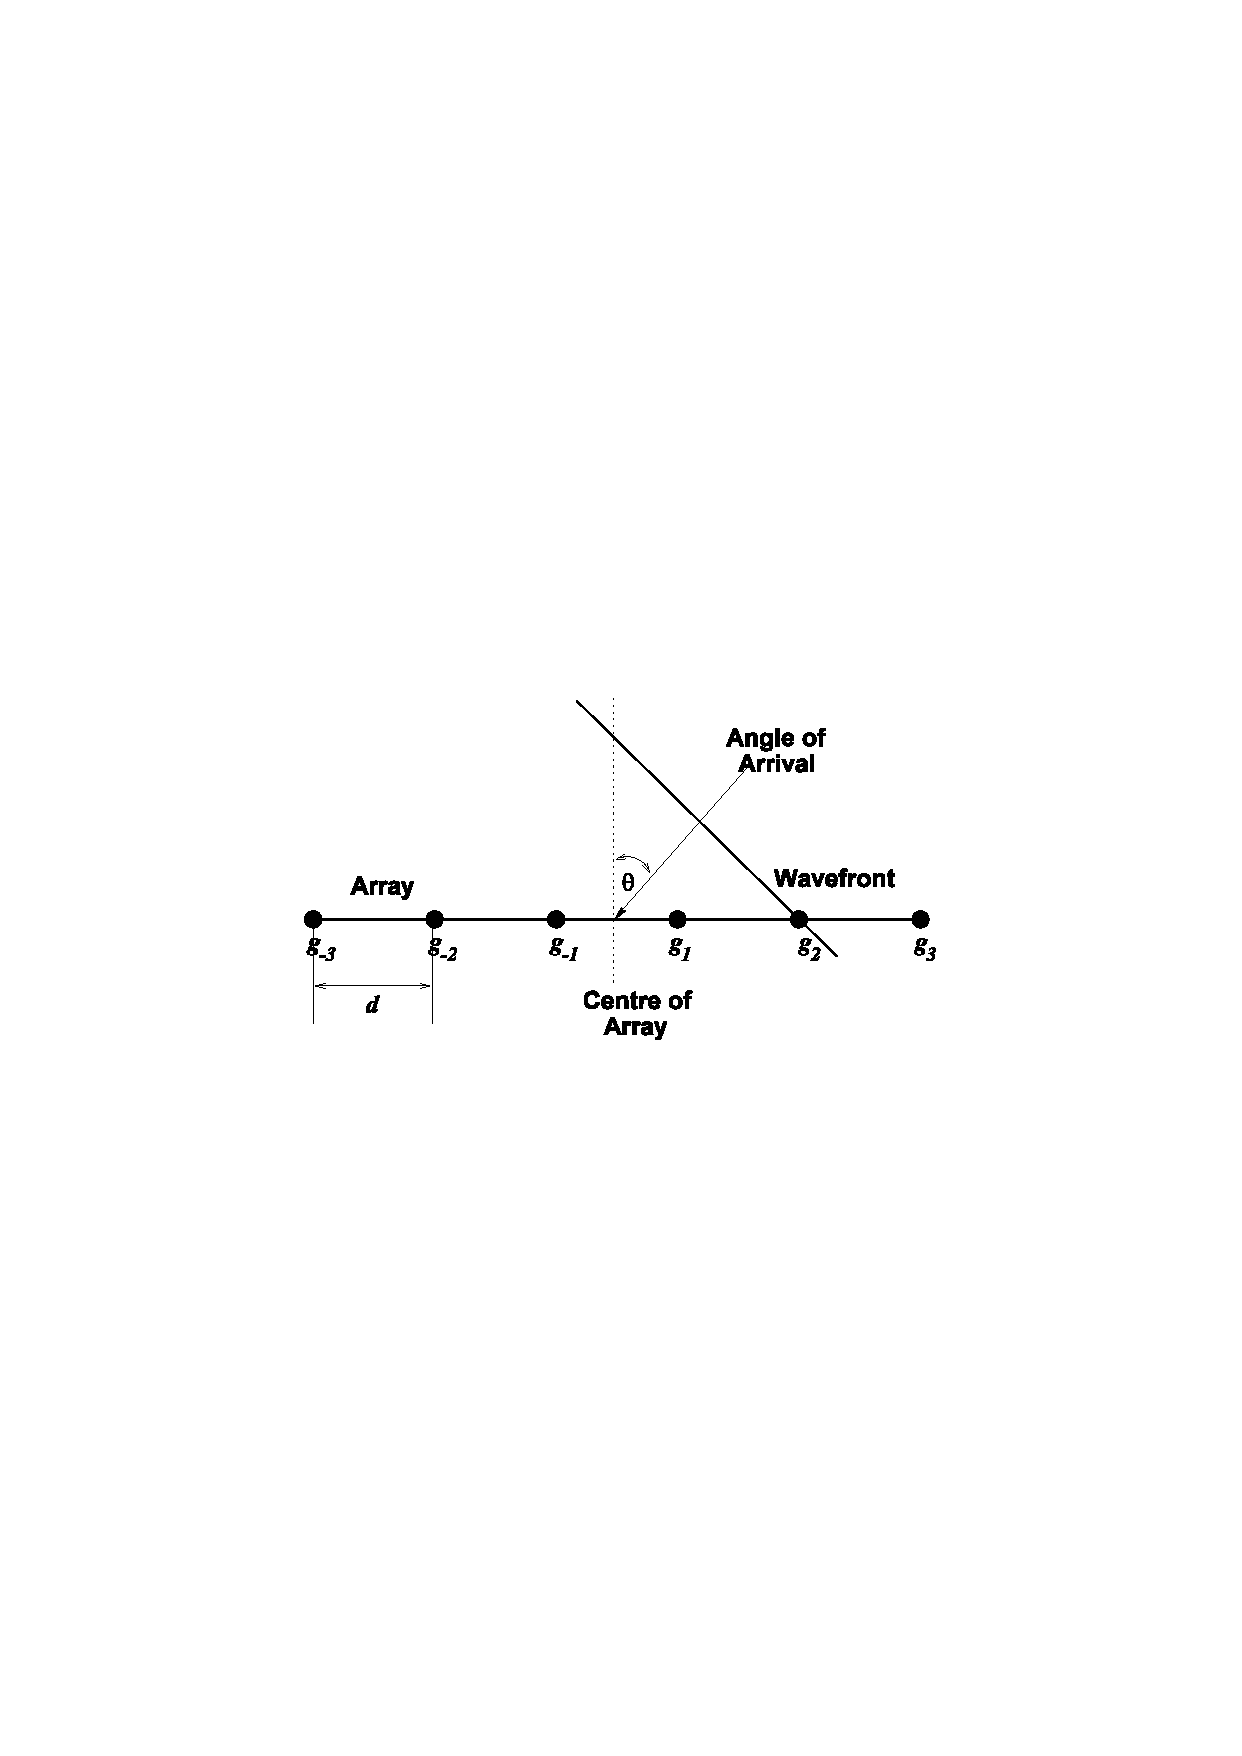
\includegraphics[trim = 50.5mm 100.2mm 50.8mm 117.3mm, clip, width=10cm]{images/antenna_array}
 %\end{center} 
 %\vspace{-1cm}
 %\caption{A uniform linear antenna array showing the angle of arrival of an incoming planar wavefront.}
% \label{fig:antenna_array}
%\end{figure}

\section{Direct Digital Synthesiser based VHF Tranceiver}

The DDS chosen is AD9854 from Analog Devices

The board used in specific is the 



\section{Current application of AD9854 DDS}




\section{Approach - Raspberry Pi driven DDS}

The aim of this project is to design of a low-cost radio transceiver of 70MHz, using the AD9854 Direct Digital Synthesiser and Raspberry Pi. The programming of synced signal will be done in C language. The transmission of samples is uniform in time.
The I and Q synthesizer function, or the RF signal, used for this research topic is: 

\begin{equation}
I(t)\cos(\omega t)+Q(t)\sin(\omega t)
\end{equation}

For signal receiver, the version 3 RTL-SDR radio receiver dongle will be used, which samples a radio frequency signal from 50 MHz to 1700MHz and outputs interleaved 8-bit IQ samples at s symbol rate up to 2.4Msps.




\section{Project scope and requirement}
Project Scope: The work performed to deliver a product, service or result with the specified features and functions. 
Requirement: A condition or capability that is required to be present in a product, service or result to satisfy a contract or other formally imposed specification.
This project is focused on implementing a transceiver with the mentioned components using knowledge on how an IQ modulator works and how to program the synced signals in C. 
There was no previous attempt on using AD9854 DDS in combination with the Raspberry Pi to implement a transceiver, hence this might be the biggest challenge. The feasibility of this design is to be analysed during the progress. There may be incompatibility between Raspberry Pi and AD9854 and this will be determined whether an issue in primary stages.



\section{Project Objective}
The project objective is to learn how an IQ modulator works and how to program synthesised signals in C programming language.
Furthermore, the cost of the design is to be kept low.



\section{Organization of thesis}

The aim of this thesis is to present the 
Chapter 1 presents the purpose of building a low-cost VHF transceiver, and the current 
Chapter 2
Chapter 3
Chapter 4






  % include the file chapter1.tex
  \chapter{Basis of RF Signal Transmission}
\vspace{-1.4em}


\section{RF Signal}




\section{Related Work}



  \chapter{Implementation of Transceiver}
\vspace{-1.4em}



\section{Components}




\section{Transmitter Implementation}




\section{Receiver Implementation}





\section{System Integration}

  \chapter{Outcome and Validation}
\vspace{-1.4em}



\section{Outcome}




\section{Validation}






\section{Discussion}
  \chapter{Conclusion and Future work}
\vspace{-1.4em}

  \chapter{Conclusions and Further Work}
\vspace{-1.4em}


  %%%%%%%%%%%%%%%%%%%%%%%%%%%%%%%
  %      Appendix
  %%%%%%%%%%%%%%%%%%%%%%%%%%%%%%%
  \appendix
  \renewcommand{\chaptermark}[1]{\markboth{Appendix \thechapter\ #1}{}}
  \chapter{$<$A Appendix Subject$>$}

  \chapter{$<$Another Appendix Subject$>$}

  
  
  %%%%%%%%%%%%%%%%%%%%%%%%%%%%%%%
  %      Bibliography
  %%%%%%%%%%%%%%%%%%%%%%%%%%%%%%%
  \renewcommand{\bibsection}{}
  \chapter*{Bibliography}
  \addcontentsline{toc}{chapter}{Bibliography}
  \bibliography{bibliography/bibliography}{}


\end{document}
